\subsubsection{Parser}
Damit die Daten im Simulink in sinnvoller Struktur verfügbar sind, muss der Inhalt entpackt werden. Dazu ist momentan die Struktur der Daten nötig. Falls die Paket ID implementiert wäre, könnte man anhand der gesetzten ID-Bits diese entpacken. Diese Aufgabe übernimmt ein 'Interpreted MATLAB Function' Block. 


\begin{lstlisting}
function output_args = parser_small(input_args)

global pck_length;

% Parse package length
pck_length = input_args(1,:);
pck_length = pck_length + 256*input_args(2,:);

% Parse package ID


% Parse package payload and convert
time = double(typecast(uint8(input_args(3:10)), 'uint64'))/1e6;
g_x = double(typecast(uint8(input_args(207:210)), 'single'));
g_y = double(typecast(uint8(input_args(211:214)), 'single'));
g_z = double(typecast(uint8(input_args(215:218)), 'single'));    

% crc detector


% output data
output_args = [time ; g_x ; g_y ; g_z ];            
\end{lstlisting}
\medskip

\noindent Der Parser muss folgende Aufgaben übernehmen:
\begin{table}[ht]
\begin{center}
  \begin{tabular}{| l | l | }
    \hline
    Zeile & Aktion \\
    \hline
    6...7  & Paketlänge zusammensetzten \\
    \hline
    10  & ID auslesen \\
    \hline
    13..16  & Nutzdaten auslesen und casten \\
    \hline
    19  & CRC16 Überprüfung der Nutzdaten \\
    \hline 
    22  & Vektorausgabe der Werte \\
    \hline 
  \end{tabular}
  
  \caption{Simulink Parser}
  \label{tab:Simulink Parser}
  
\end{center}
\end{table}



%\begin{figure}[ht]
%  \begin{center}
%  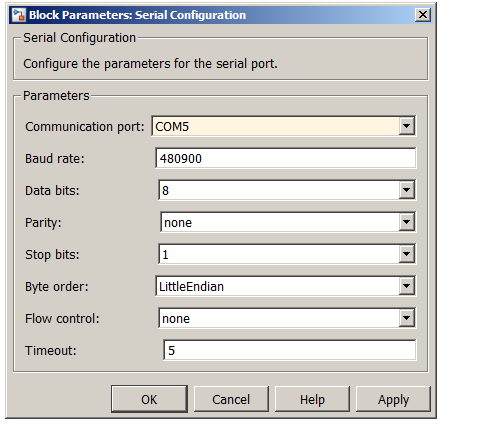
\includegraphics[width=0.5\textwidth]{pic/60_simulink/conf_conf.png}
%  \caption{tmp}
%  \label{fig:temp}
%  \end{center}
%\end{figure}


\clearpage